\chapter{A Theory about Propositional Logic} \label{meta}

In Chapter \ref{theories}, we talked about how to formulate theories
in predicate logic.  Now here's a weird idea: how about we formulate a
theory (in predicate logic) about propositional logic?  Think of it
this way.  Suppose that you travel far back in time, to a time when
human beings didn't know how to reason with quantifiers --- they only
knew how to reason with the propositional connectives ``and'', ``or'',
etc.\footnote{As far as I know, nobody believes that's how human
  thinking actually evolved.}  Your job is to describe the rules of
the ``game'' that these early, propositional-logical humans like to
play.

If you think that the scenario we've just described is strange or
silly, then just think of it as a warm up for the real job: looking in
the mirror, i.e.\ reasoning about how we reason.  Obviously, good
human thinking isn't exhausted by propositional logic; at the very
least, it also involves inferences with quantified statements.  Hence,
we'll want eventually to have a theory about predicate logic.  We'll
turn to that in Chapter \ref{meta2}, and we'll restrict ourselves in
this chapter to propositional logic.

So, to return to our simplified and fictional set up: we want a theory
$T$ that describes propositional logic.  To build $T$, we first need
to decide on a vocabulary, i.e.\ on relation symbols, function
symbols, names, etc.\ that can be used to describe propositional
reasoning.  For this, we'll make use of set theory.  We will assume
that there is a non-empty set $\Sigma$, which we'll call the
\glspl{atomic sentence}.  To be clear, the things in $\Sigma$ aren't
{\it our} atomic sentences --- i.e.\ they aren't part of our language.
Instead of using the sentences in $\Sigma$, we are talking {\it about}
them.  We also assume that there is another set containing the symbols
$\wedge,\vee ,\to,\neg$, and perhaps some parentheses.  Again, don't
think of those symbols as the logical connectives we use; instead,
they are the logical connectives that are used by the people we are
studying.  Finally, we assume that there is a basic operation on
symbols called ``concatenation.'' \label{formation}

We then notice that the people we are studying treat some strings of
symbols differently than others.  We then hypothesize that there is a
feature of strings, which we might call ``sentencehood,'' and we
introduce a predicate symbol $\mathsf{sent}(\phi )$ to our language
that we will use to describe which things are sentences.  (Here we're
using Greek letters, such as $\phi$, as our variables.)  Here then is
our theory about the grammar of propositional logic:
\begin{itemize}
\item Any symbol in the set $\Sigma$ is a sentence.  
\item For any string $\phi$ of symbols, if $\phi$ is a sentence, then
  so is the string $\neg \phi$.
\item If $\phi$ and $\psi$ are sentences, then $\phi\vee\psi$ is a
  sentence.
\item If $\phi$ and $\psi$ are sentences, then $\phi\wedge\psi$ is a
  sentence.
\item If $\phi$ and $\psi$ are sentences, then $\phi\to\psi$ is a
  sentence.
\end{itemize}
All of these axioms seem obviously correct, but they are not yet
sufficient, for they don't entail some other things we know --- for
example, that our test subjects do {\it not} count gibberish strings
as sentences.  To capture that additional claim, we draw upon a little
bit of set theory to say that the set of sentences is like the set of
natural numbers, viz.\ all of its elements result from a finite number
of applications of the construction methods to the atomic sentences.

We can give a visual representation of the construction of a sentence
by means of the notion of a \emph{parse tree}.  In such a tree, each
node corresponds to a formula.  The initial nodes must be atomic
sentences; and new nodes can be constructed from old ones using the
propositional connectives.  Thus, for example, given nodes $\phi$ and
$\psi$ we can construct new nodes as follows:
\[ \begin{tikzcd}
  \neg\phi\arrow[-]{d} & & & \phi\wedge \psi \arrow[-]{dl} \arrow[-]{dr} \\
  \phi & & \phi & & \psi \end{tikzcd} \]
Here's one example of a full parse tree:
\[ \begin{tikzcd}
    & & \neg (P\wedge Q)\to R \arrow[-]{dl} \arrow[-]{dr} & & \\
    & \neg (P\wedge Q) \arrow[-]{d} & & R & \\
    & P\wedge Q \arrow[-]{dl} \arrow[-]{dr}       & &  & \\
    P & & Q & & \end{tikzcd} \] Parse parse trees are useful in many
ways.  First, a parse tree allows us to define the notion of a
\gls{subformula} of a formula $\phi$: namely, any formula that occurs
in the parse tree of $\phi$.  Second, a parse tree provides a nice
visual representation of how the truth-value of a sentence $\phi$ is
computed from the truth-value of its atomic subformulas.  Indeed, each
node of a parse tree can be considered as a logic circuit: a negation
node is the $\mathsf{not}$ circuit that flips a bit, a conjunction
node is the $\mathsf{and}$ circuit that gives output $1$ only if both
inputs are $1$, etc.  Third, a parse tree makes it obvious what the
\gls{main connective} of a sentence is: it's the connective at the
root node of the parse tree.  Finally, parse trees give a nice visual
picture of what happens during \gls{substitution}.  Consider the
simple case of the substitution $F(P)=Q\to R$ and
$F(Q)=R\wedge \neg R$ applied to the sentence $\phi\equiv P\to Q$.
The parse tree of $F(\phi )$ results from simply pasting the trees for
$F(P)$ and $F(Q)$ to the nodes for $P$ and $Q$ in the parse tree of
$P\to Q$.
\[ \begin{tikzcd}
    & P\to Q \arrow[-]{dl} \arrow[-]{dr} &    & & F(P\to Q)\equiv (Q\to R)\to
    (R\wedge\neg R) \arrow[-]{dl} \arrow[-]{dr} & \\
  P &        & Q  & F(P) &                    & F(Q) 
\end{tikzcd} \] 

\section{Induction on the construction of sentences}

In Chapter \ref{theories}, we saw that the set $N$ of natural numbers
is defined so as to license the method of ``proof by induction.''
This method says, roughly, that if you can prove that $0$ is $\phi$,
and if you can prove that whenever $n$ is $\phi$ then so is $n+1$,
then it follows that all natural numbers are $\phi$.  We will now see
that this method of proof can be adapted to the set of sentences of
propositional logic --- giving us a powerful tool for proving that
something or other is true for all sentences.

% Let $<$ be a binary relation, and let $T$ be a theory which says that
% $<$ is a linear order that has a least element, and such that for
% every element, there is a unique succeeding element.  We can capture
% the latter requirement with the axiom:
% \[ \forall x\exists y\forall z((x<z)\leftrightarrow (y\leq z)) \] Of
% course, we're very familiar with structures of the sort described by
% $T$, in particular the natural numbers $0,1,2,\dots $.

% Before proceeding, let's note that the theory $T$ permits us to define
% some new concepts.  In particular, $T$ says that for each element,
% there is a unique element that immediately succeeds it.  To be more
% precise, consider the relation:
% \[ \theta (x,y) \: \equiv \: (x<y)\wedge \neg \exists z((x<z)\wedge
% (z<x)) .\] Then $T\vdash \forall x\exists !y\theta (x,y)$, and we can
% introduce a function symbol $s(x)$ to denote the unique $y$ such that
% $\theta (x,y)$.

% Now suppose that $p$ is a predicate symbol, consider the following sequent:
% \[ p(0) , \;\forall x(p(x)\to p(s(x))) \:\vdash\: \forall xp(x) \qquad
% (*) \] Is (*) valid?  That's not an easy question to answer.  But in
% fact, it is \emph{not} valid, as the following example shows: take the
% natural numbers $0,1,2,\dots $, but then add to the end of the natural
% numbers a copy of all integers, negative and positive.  In other
% words, consider the ordered set $M$:
% \[ 0,1,2,\dots ,-1',0',1',\dots , \] where each ellipsis indicates an
% infinite number of succeeding elements.  Let's also stipulate that the
% predicate $p$ applies to an element $x$ of $M$ just in case $x$ is a
% member of the first sequence of natural numbers.  Then $T$ is true in
% $M$, and the premises of (*) are true in $M$; but the conclusion of
% (*) is \emph{false} in $M$.  Therefore, the sequent (*) is not
% logically valid.

% Nonetheless, there are cases where we'll want to assume the validity
% of (*).  These are cases where we've constructed a collection $S$, and
% where we want then to prove that everything in $S$ has a certain
% feature $\phi$.  The most notable cases of such collections are:
% natural numbers $0,1,2,\dots $, sentences of propositional logic, and
% sequents of propositional logic.

% %% TO DO: first talk about induction on natural numbers ,e.g. $\Sum n$
% %% ...

Let $\Sigma$ be a fixed set of atomic sentences.  For simplicity,
we'll first consider a simple case where $\Sigma = \{ P \}$, and where
$\Delta$ is the set of sentences that are built with the $\neg$ and $\vee$
connectives.  If you think of the set of sentences on analogy to the
natural numbers $N$, then the sentence $P$ is the $0$, and the
connectives $\neg$ and $\vee$ are like the successor function.  In the
case of the set $N$ of natural numbers, each number $n\in N$ is the
result of applying the successor function $s$ to $0$ some finite
number of times.  In the case of the set $\Delta$ of sentences, each
sentence $\phi\in \Delta$ results from taking a certain number of copies of
$P$, and applying the connectives $\neg$ and $\vee$ a finite number of
times.  This definition of the set $\Delta$ thus licenses the following
extension of the method of proof by induction.

\bigskip \begin{tcolorbox}[enhanced,width=11cm,title=Induction on the
  construction of sentences,attach boxed title to top
  left={yshift=-2mm,xshift=4mm},boxed title style={sharp corners}]
  \[ \begin{array}{c p{6cm} p{2.2cm}}
       (1) & Atomic sentences have property $X$. & base case \\
       (2) & If $\phi$ and $\psi$ have property
             $X$, then $\phi\vee\psi$ has
             property $X$. & induction $\vee$ \\
       (3) & If $\phi$ has property $X$, then
             $\neg\phi$ has property $X$. & induction
                                            $\neg$ \\ \hline
       (\text{C}) & Every sentence in $\Delta$ has property
                    $X$. & conclusion \end{array} \] \end{tcolorbox}
 \bigskip What we have here is a family of inference rules, one for
 each property $X$ that can be described in our meta-theory of
 propositional logic.  We haven't been completely precise in telling
 which properties of sentences can be articulated.  However, as a
 general rule, the only relevant properties are the {\it purely
   syntactic} properties, e.g.\ ``the main connective of $\phi$ is $\wedge$,'' or ``$\phi$ has three left parentheses.''

We'll now use induction to show that every sentence in $\Delta$ is
provably equivalent to one of the four in the diamond:
\[ \begin{tikzcd} & \arrow[-]{dl} \top \arrow[-]{dr} & \\
    P & & \neg P \\
    & \arrow[-]{ul} \bot \arrow[-]{ur} & \end{tikzcd} \] Here $\top$
is shorthand for some tautology, e.g.\ $P\vee\neg P$, and $\bot$ is
shorthand for some contradiction, e.g.\ $P\wedge\neg P$, and to say
that $\phi$ and $\psi$ are \emph{provably equivalent} just means that
$\phi\dashv\vdash\psi$.

\begin{prop} Every sentence in $\Delta$ is provably equivalent to one of
   the four in the diamond above.
\end{prop}

 Before we start the official proof, observe that if $\phi$ and $\psi$
 are provably equivalent, then so are $\neg\phi$ and $\neg\psi$.
 Indeed, suppose we're given proofs $\phi\vdash\psi$ and
 $\psi\vdash\phi$.  Then we can obtain proofs of
 $\neg\phi\vdash\neg\psi$ and $\neg\psi\vdash\neg\phi$ by using the
 (derived) contrapositive rule.  Similarly, if $\phi$ and $\phi '$ are
 provably equivalent, and $\psi$ and $\psi '$ are provably equivalent,
 then so are $\phi\vee\psi$ and $\phi '\vee\psi
 '$.

 \begin{exercise} Prove that if $\phi\dashv\vdash\phi '$ and
   $\psi\dashv\vdash\psi '$ then
   $(\phi\vee\psi )\dashv\vdash (\phi '\vee\psi ')$. \end{exercise}
 
 \begin{proof}  \fbox{base case} \, Obviously $P$ is equivalent to itself, hence it's
   equivalent to one of the four sentences in the diamond.

   \bigskip \noindent \fbox{induction $\neg$} \, Suppose that $\phi$ is equivalent to one of
   the four in the diamond.  If $\phi$ is equivalent to $\top$, then
   $\neg\phi$ is equivalent to $\bot$.  If $\phi$ is equivalent to
   $P$, then $\neg\phi$ is equivalent to $\neg P$.  Etc.

   \bigskip \noindent \fbox{induction $\vee$} \, Suppose that $\phi$
   and $\psi$ are each equivalent to some sentence in the diamond.  If
   $\phi$ is equivalent to $\bot$, then $\phi\vee\psi$ is equivalent
   to $\psi$.  If $\phi$ is equivalent to $\top$, then $\phi\vee\psi$
   is equivalent to $\top$.  Similar conclusions hold if $\psi$ is
   equivalent to $\top$ or $\bot$.  If $\phi$ and $\psi$ are
   equivalent to each other, then $\phi\vee\psi$ is equivalent to
   $\phi$.  Finally, if $\phi$ is equivalent to $\neg\psi$, then
   $\phi\vee\psi$ is equivalent to $\top$.
 \end{proof}

We've seen how to use proof by induction to show that something is
true for every sentence in the set $\Delta$ of sentences containing only
the connectives $\vee$ and $\neg$.  This method can now be extended to
the set of {\it all} sentences, only we need to add inductive steps
for the other two connectives, $\wedge$ and $\to$.
\[ \begin{array}{c p{5cm} p{2.2cm}}
(4) & If $\phi$ and $\psi$ have property $X$, then $\phi\wedge\psi$ has
     property $X$. & induction $\wedge$ \\
(5) & If $\phi$ and $\psi$ have property $X$, then $\phi\to\psi$ has
     property $X$.  & induction $\to$ \end{array} \]
We will now use induction to prove that every sentence (whose only
atomic sentence is $P$) is equivalent to one of the four in the
diamond.  We have already shown that every sentence in $\Delta$ is
equivalent to one of the four in the diamond.  Thus, it will suffice
--- by the transitivity of logical equivalence --- to show that every
sentence is equivalent to a sentence in the set $\Delta$.     
 
\begin{prop} Every sentence is provably equivalent to a sentence in
  the set $\Delta$.  \end{prop}

\begin{proof} Let's say that a sentence $\phi$ has property $X$ just
  in case $\phi$ is provably equivalent to a sentence in the set
  $\Delta$.  We will use induction on the construction of formulas to
  prove that every sentence has property $X$.  Before we begin, note
  that if $\psi$ has property $X$, and \mbox{$\phi\dashv\vdash\psi$},
  then $\phi$ has property $X$.

  \bigskip \noindent \fbox{base case} \, Since $P\in\Delta$, $P$ has
  property $X$.

  \bigskip \noindent \fbox{induction $\vee$ and $\neg$} \, If $\phi$
  and $\psi$ have property $X$, then $\neg \phi$ and $\phi\vee\psi$
  obviously have property $X$.

  \bigskip \noindent \fbox{induction $\wedge$} \, Suppose that both
  $\phi$ and $\psi$ have property $X$.  Then
  $\phi\wedge\psi\dashv\vdash\neg (\neg\phi\vee\neg\psi )$, and the latter
  obviously has property $X$.  Therefore, $\phi\wedge\psi$ has
  property $X$.

  \bigskip \noindent \fbox{induction $\to$} \, Suppose that both
  $\phi$ and $\psi$ have property $X$.  Then
  $\phi\to\psi\dashv\vdash\neg\phi\vee\psi$, and the latter obviously has
  property $X$.  Therefore, $\phi\to\psi$ has property $X$.

  \bigskip \noindent This completes the inductive steps, and so it
  follows that every sentence has property $X$.
\end{proof}

\begin{exercise} Let $\Theta$ be the set of sentences whose only
  atomic sentence is $P$, and whose only connectives are $\neg$ and
  $\wedge$.  Show that every sentence is provably equivalent to a
  sentence in $\Theta$. \end{exercise}

\begin{exercise} Let $\Gamma$ be the set of formulas defined as follows:
  \begin{itemize}
  \item $P\in \Gamma$,
  \item If $\phi\in\Gamma$ and $\psi\in\Gamma$ then
    $\phi\vee\psi\in\Gamma$;
  \item Every element of $\Gamma$ arises from a finite number of the
    previous steps.
  \end{itemize} Use mathematical induction to show that for all
  $\phi\in\Gamma$, $\phi\vdash P$.
\end{exercise}  


\section{Truth Functions}

In Chapter \ref{truth} we introduced truth-tables as a tool for
deciding whether arguments are valid or not.  It's time now to think
more theoretically about what truth-tables are, and about what they
can do.

Each one of our connectives $\neg ,\wedge ,\vee$ and $\to$ has an
associated truth-table.  Therefore, these connectives are
\emph{\gls{truth-functional}}, i.e.\ the truth-value of an output
sentence, say $\neg \phi$, is completely determined by the truth-value
of the input sentence $\phi$.  Now, you might wonder: how in the world
could a connective {\it not} be truth-functional?  Well, consider for
example, the connective, ``Donald Trump said that \dots ''.  This
phrase is a bona fide propositional connective because for any
declarative sentence $\phi$, you can set it in the blank, and the
output is a new sentence: ``Donald Trump said that $\phi$.''  However,
even the most blind defender of Trump wouldn't want to say that this
connective is truth-functional, for there is surely at least one false
sentence $\phi$ such that ``Donald Trump said that $\phi$'' is true,
and at least one false sentence $\psi$ such that ``Donald Trump said
that $\psi$'' is false.  Therefore, the connective cannot determine
the output truth-value simply on the basis of the input truth-value.

The ``Donald Trump said that \dots '' connective has not been studied
carefully by philosophers.  However, there are other
non-truth-functional connectives that have been.  One of philosophers'
favorites is the connective ``It is necessarily true that \dots ''.
As long as there are some truths that are not necessarily true, then
this connective is not truth-functional.  And since philosophers have
long been interested in necessary truths, they have taken particular
interest in non-truth-functional connectives.  They study these
connectives in a subject called \emph{modal logic}.

Our focus here, however, is on truth-functional connectives.  We can
now raise the question: are there other truth-functional connectives
besides $\neg ,\vee ,\wedge ,\to$?  Well, immediately we know the
answer is yes, for we also have the connective $\lra$, which doesn't
have the same truth table as any of those latter three.  However, you
might be quick to point out that the truth table for $\lra$ can be
simulated by using both the $\wedge$ and $\to$ connectives.  Let's
distinguish then between connectives that can be expressed in terms of
$\neg ,\vee ,\wedge ,\to$, and those that cannot be so expressed.  We
can then rephrase the question as: are there any truth-functional
connectives that cannot be expressed in terms of the ones we already
have?

It might sound at first like that question is impossibly difficult to
answer.  But let's start by thinking about how many possible
truth-functions there could be.  (Here a \emph{truth-function} is
simply a function that takes truth-values as inputs, and returns
truth-values as outputs.  Since our truth-values are $0$ and $1$, a
truth-function is a function from the set $\{ 0,1\}$ to itself.)  For
this, we need to do some basic calculation.  Starting with the case of
unary truth-functions (i.e.\ those that take one input), there are
precisely $4$ functions from $\{ 0,1\}$ to itself: the identity
function, the function that exchanges $0$ and $1$, the function that
maps both elements to $0$, and the function that maps both elements to
$1$.  And clearly we can express those four functions in terms of
combinations of connectives, e.g.\ the constant $0$ function is
expressed by $P\wedge\neg P$.

Now, for binary truth-functions (i.e.\ those with two inputs), we
already have many more possibilities.  Each function from
$\{ 0,1\}\times \{ 0,1\}$ to $\{ 0,1\}$ corresponds to a division of
the former set into two parts: those elements that get assigned $0$,
and those elements that get assigned $1$.  Since the former subset is
the complement of the latter, each such function is uniquely
determined by the subset of elements to which it assigns $1$.  Hence,
there is a one-to-one correspondence between binary truth-functions
and subsets of $\{ 0,1\}\times \{ 0,1\}$, i.e.\ elements of the
powerset of $\{ 0,1\}\times\{ 0,1\}$.

If a set $X$ has $|X|$ elements, then $X$ has $2^{|X|}$ subsets.  In
the case at hand, $\{ 0,1\}\times \{ 0,1\}$ has $4$ elements, hence
$2^4$ subsets; consequently, there are $2^4=16$ binary
truth-functions.  Thus, there are $13$ more truth-functions besides
those represented by $\wedge ,\vee$ and $\to$.  It might seem, then,
we're very far indeed from being able to express all binary
truth-functions.  But in fact, the opposite is true.  In Figure
\ref{hasse}, we display $16$ sentences that have distinct truth tables.
%% TO DO: fix this ugly table
\begin{figure}[htbp]
  \centering
  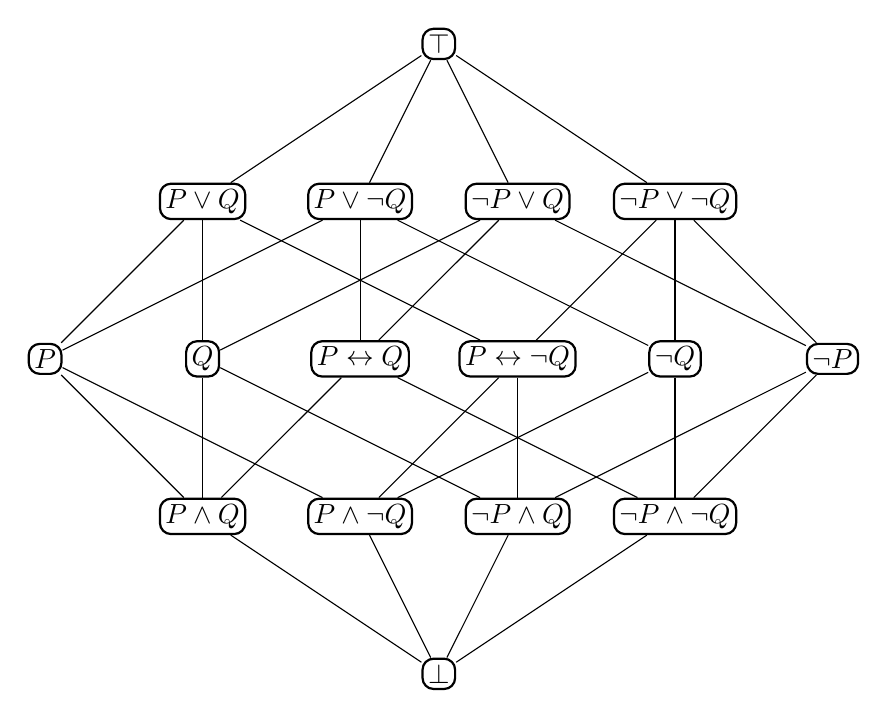
\begin{tikzpicture}[source/.style={draw,thick,rounded corners,inner sep=2pt}]
\node[source] (min) at (0,-1) {$\bot$};
\node[source] (A1) at (-3,1) {$P\wedge Q$};
\node[source] (A2) at (-1,1) {$P\wedge \neg Q$};
\node[source] (A3) at (1,1) {$\neg P\wedge Q$};
\node[source] (A4) at (3,1) {$\neg P\wedge \neg Q$};
\node[source] (B1) at (-5,3) {$P$};
\node[source] (B2) at (-3,3) {$Q$};
\node[source] (B3) at (-1,3) {$P\leftrightarrow Q$};
\node[source] (B4) at (1,3) {$P\leftrightarrow \neg Q$};
\node[source] (B7) at (3,3) {$\neg Q$};
\node[source] (B8) at (5,3) {$\neg P$};
\node[source] (C1) at (-3,5) {$P\vee Q$};
\node[source] (C2) at (-1,5) {$P\vee \neg Q$};
\node[source] (C3) at (1,5) {$\neg P\vee Q$};
\node[source] (C4) at (3,5) {$\neg P\vee \neg Q$};
\node[source] (max) at (0,7) {$\top$};
\draw (min) -- (A1);
\draw (min) -- (A2);
\draw (min) -- (A3);
\draw (min) -- (A4);
\draw (A1) -- (B1);
\draw (A1) -- (B3);
\draw (A1) -- (B2);
\draw (A2) -- (B1);
\draw (A2) -- (B4);
\draw (A2) -- (B7);
\draw (A3) -- (B2);
\draw (A3) -- (B4);
\draw (A3) -- (B8);
\draw (A4) -- (B3);
\draw (A4) -- (B8);
\draw (A4) -- (B7);
\draw (B1) -- (C1);
\draw (B1) -- (C2);
\draw (B2) -- (C1);
\draw (B2) -- (C3);
\draw (B3) -- (C2);
\draw (B3) -- (C3);
\draw (B4) -- (C1);
\draw (B4) -- (C4);
\draw (B7) -- (C2);
\draw (B7) -- (C4);
\draw (B8) -- (C3);
\draw (B8) -- (C4);
\draw (C1) -- (max);
\draw (C2) -- (max);
\draw (C3) -- (max);
\draw (C4) -- (max);
\end{tikzpicture}
\caption{Horizontal rows have the same number of $1$'s.  A connecting line indicates logical implication going upwards.} \label{hasse} 
\end{figure}

Since we have equivalences:
\[ P\to Q \equiv \neg P\vee Q \qquad \text{and} \qquad P\wedge Q
  \equiv \neg (\neg P\vee \neg Q) , \] any sentence is equivalent to a
sentence whose only connectives are $\vee$ and $\neg$, and each of the $16$ truth
functions can be expressed in terms of these connectives.  Similarly,
each of these $16$ truth functions can be expressed just with $\neg$
and $\wedge$.  If every truth-function
can be expressed in terms of a set $\Gamma$ of connectives, then we
say that $\Gamma$ is \emph{\gls{expressively complete}} or
\emph{expressively adequate}.  Thus, we just sketched proofs that
$\{ \neg ,\vee\}$ and $\{ \neg ,\wedge\}$ are expressively complete.

Amazingly, there is a single truth-function that is itself
expressively complete.  The corresponding connective is called
``nand'', and is usually symbolized by $\uparrow$.  The truth-table
for $P \uparrow Q$ is, by definition, the same as that for
$\neg (P\wedge Q)$.
\[ \begin{array}{ c@{\, }c | c@{\, }c@{\, }c }
P & Q   & P & \uparrow & Q  \\  \hline
1 & 1   & 1 & \mathbf{0} & 1  \\
1 & 0   & 1 & \mathbf{1} & 0  \\
0 & 1   & 0 & \mathbf{1} & 1  \\
0 & 0   & 0 & \mathbf{1} & 0  \\
\end{array} \]
To show that the set $\{ \uparrow \}$ is expressively complete, it will suffice
to show that it can reproduce the truth tables for $\neg$ and $\vee$.
After some trial and error, we find that the following definitions work:
\[ \begin{array}{c c c c } \begin{array}{ c | c@{\, }c@{\, }c}
P & P & \uparrow & P  \\
\hline 
1 &   1 & \mathbf{0} & 1  \\
0 &   0 & \mathbf{1} & 0  \end{array} 
& & & \begin{array}{ c@{\, }c | c@{ }c@{\, }c@{\, }c@{ }c@{\, }c@{\, }c@{ }c@{\, }c@{\, }c@{ }c@{ }c@{ }c}
     P & Q &   ( & P & \uparrow & P & ) & \uparrow & ( & Q & \uparrow & Q & ) & \\
\hline 
1 & 1 &    & 1 & 0 & 1 &  & \mathbf{1} &  & 1 & 0 & 1 &  & \\
1 & 0 &    & 1 & 0 & 1 &  & \mathbf{1} &  & 0 & 1 & 0 &  & \\
0 & 1 &    & 0 & 1 & 0 &  & \mathbf{1} &  & 1 & 0 & 1 &  & \\
0 & 0 &    & 0 & 1 & 0 &  & \mathbf{0} &  & 0 & 1 & 0 &  & \\
      \end{array} \end{array} \]
  \begin{exercise} Give a formula using only $P,Q$ and $\uparrow$ that
    has the same truth-table as $P\wedge Q$. \end{exercise} If any
  truth-function can be expressed by the $\uparrow$ connective, then, why, you might wonder, don't we 
  use it, instead of the redundant collection $\{ \neg ,\vee ,\wedge
  ,\to \}$ of four connectives?  The answer, in short, is that we
  face a trade off between simplicity and naturality, where the latter
  is a function of what we are familiar with.  For most of us, it's
  fairly natural to reason in terms of ``and'', and less natural to
  reason in terms of ``nand''.  Why that is, we don't pretend to know.
  Nonetheless, you now know that if somebody has the concept of
  ``nand'', then they can express any other truth-functional concept.

It can be more difficult to show that a set of connectives is {\it
  not} expressively complete.  For example, suppose that we want to
show that the set $\{ \vee \}$ is not, by itself, truth-functionally
complete.  The way we would approach this is to start trying to
express some of the truth-tables, to get a feeling of what we {\it
  cannot} do.  With the connective $\vee$, we can write $P\vee P$,
which is equivalent to $P$ again.  We can also write $P\vee Q$.  But
it seems that we get stuck at that point.  If we write longer
disjunctions, say $P\vee (P\vee Q)$, we quickly realize that we
haven't expressed anything new.  That is, we get stuck with
truth-functions that are true whenever $P$ and $Q$ are true.  That
realization then gives us an idea: perhaps we can prove that every
truth-function that can be expressed with just $\vee$ has this
feature, i.e.\ that it's true whenever $P$ and $Q$ are true.  That
idea provides the intuition behind the following proof.

  To make this proof a bit more clear, we need a slight change of
  terminology.  Instead of talking about a row of a truth-table, let's
  talk about a \emph{valuation}.  To be precise, a valuation $v$
  assigns each atomic sentence (in this case, $P$ and $Q$) either $0$
  or $1$.  If we follow the truth-table recipe, then a valuation
  naturally extends to assign every sentence either $0$ or $1$.  For
  example, if $v(\phi )=1$ and $v(\psi )=1$ then $v(\phi\vee\psi
  )=1$.  The claim above, then, is that if $v$ is a valuation such
  that $v(P)=1$ and $v(Q)=1$, then $v(\phi )=1$ for any sentence whose
  only connective is $\vee$. 

\begin{prop} The set $\{ \vee\}$ is not truth-functionally
  complete. \end{prop}

\begin{proof} Let $\Gamma$ be the set of sentences built only with the
  connective $\vee$.  Let $v$ be the valuation that assigns $1$ to
  every atomic sentence.  We show that for every sentence
  $\phi\in\Gamma$, $v(\phi )=1$.  Our argument proceeds by induction
  on the construction of $\Gamma$.  By definition, for $\phi$ an
  atomic sentence in $\Gamma$, we have $v(\phi )=1$.  Furthermore, if
  $v(\phi )=1$ and $\phi (\psi )=1$ then $v(\phi\vee\psi )=1$.
  Therefore, $v(\phi )=1$ for all $\phi\in \Gamma$.  It follows that
  there is no sentence in $\Gamma$ that is logically equivalent to
  $P\wedge\neg P$, and $\{ \vee \}$ is not truth-functionally
  complete.
\end{proof}

\begin{exercise} 
Show that the set $\{ \wedge \}$ is not truth-functionally
complete. \end{exercise}
\begin{exercise} Consider sentences built out of the atomic sentences $P$ and
    $Q$.  In this case, there are four valuations $v_1,v_2,v_3,v_4$.
    Let's say that a sentence $\phi$ is a {\it even} just in case
    $\phi$ is true for either $0,2$, or $4$ valuations.  Show that if
    $\phi$ is even then $\neg \phi$ is even.  Show that if $\phi$ and
    $\psi$ are even, then $\phi\lra\psi$ is even. \end{exercise}
  \begin{exercise} Is the set $\{ \neg ,\lra \}$ truth-functionally
    complete? \end{exercise}

%% TO DO: draw sentences as subsets of the space of valuations

%% TO DO: prove $\vdash (P\lra Q)\vee (P\lra R)\vee (P\lra R)

%% TO DO: show that $P\lra (P\lra Q)\equiv Q$





%% TO DO -- define substitution instances

\section{A theory of what can be proven}

In the previous sections we developed a theory about the grammar and
semantics of propositional logic.  In this section we develop a theory
about proofs, i.e.\ about what can and cannot be proven with the
inference rules for propositional logic.  To this end, we introduce
into {\it our} language --- i.e.\ the language we are using to
describe propositional logic --- a relation symbol $\vdash$, which we
write in infix notation, taking an argument on the left and an
argument on the right.  (Technically, the symbol $\vdash$ ambiguously
represents several different relation symbols, one for each finite
number of sentences that can occur on the left.  But we'll brush this
complication under the rug.)

The inference rules for propositional logic provide an \emph{inductive
  definition} of the set of valid sequents, i.e.\ of the extension of
the relation $\vdash$.  \index{definition!inductive} The base case
here is the rule of assumptions: for any formula $\phi$, the sequent
$\phi\vdash\phi$ is valid.  Each of the other inference rules is a
recipe for constructing a new valid sequent from one, two, or three
old ones.  Since the extension of $\vdash$ is defined inductively, it
follows that we can prove things about all sequents by means of an
induction schema.  Here the induction schema looks like this:

\bigskip \begin{tcolorbox}[enhanced,width=12cm,title=Induction on the
  construction of sequents,attach boxed title to top
  left={yshift=-2mm,xshift=4mm},boxed title style={sharp corners}]
$ \begin{array}{c p{7cm} p{2.3cm}}
     (1) & $\phi\vdash\phi$ has property $X$. & base \\
     (2) & If $\Gamma\vdash \phi\to\psi$ and
           $\Gamma\vdash\phi$ have property
           $X$, \newline then $\Gamma\vdash\psi$ has property $X$. &
                                                                     induction MP  \\
     \vdots \\ \hline
     (\text{C}) & All sequents have property
                  $X$. & conclusion \end{array} $ \end{tcolorbox} As
              you can see, a proof by induction on the construction of
              sequents will involve {\it many} inductive steps --- one
              for each inference rule.  But what kinds of things might
              we want to show about the collection of all sequents?
              There are two things about the collection of sequents
              that we've already assumed and used.  First, we assumed
              that sequents couldn't be messed up by find-and-replace
              operations.  That is, for any sequent
              $\phi\vdash\psi$, if you perform a uniform substitution
              of sentences for propositional constants, then you get
              another valid sequent $F(\phi )\vdash F(\psi )$.  Second, we assumed that truth-tables can detect when a sequent cannot be proven.  In other words, we assumed that for any valid sequent $\phi\vdash\psi$, the truth table for $\phi$ and $\psi$ will have no row in which $\phi$ is true and $\psi$ is false.  It's time now to prove that these two assumptions are true.

In order to set up these proofs, it will be helpful to imagine two
different languages, with different atomic sentences.  Let $\Sigma$ be
one list of atomic sentences, and let $\Sigma '$ be another list of
atomic sentences.  We call $\Sigma$ the \emph{\gls{signature}}
\index{signature} of the one language, whereas $\Sigma '$ is the
signature of the second language.  (If it helps you to remember, you
could think of $\Sigma '$ as having atomic sentences that have a prime
symbol, say $P',Q',R'$.)  We then let both languages build their
sentences from their respective atomic sentences using the logical
connectives $\neg ,\wedge ,\vee ,\to$.

Now let's imagine what might count as a \emph{\gls{translation}}
\index{translation} between languages $\Sigma$ and $\Sigma '$.  Keep
in mind that a good translation between languages need not be
word-for-word.  For example, it's doubtful that there is a single
English word that could translate the German word {\it Zeitgeist}, or
a single English word that could translate the Danish word {\it
  hygge}.  (I've hear that there are many more interesting examples
from languages such as Hindi, Urdu, and Mandarin.)  So, we shouldn't
require that a translation from $\Sigma$ to $\Sigma '$ has to match an
atomic sentence in $\Sigma$ with an atomic sentence in $\Sigma '$.
Instead, we will allow that an atomic sentence in $\Sigma$ be
reconstrued as {\it any} sentence of $\Sigma '$.

\begin{defn} Let $\Sigma$ and $\Sigma '$ be propositional signatures.
  A \emph{\gls{reconstrual}} $F$ from $\Sigma$ to $\Sigma '$ is a
  function that takes atomic sentences of $\Sigma$ to sentences of
  $\Sigma '$.  \end{defn}

A reconstrual $F:\Sigma\to\Sigma '$ extends naturally to a function
from {\it all} sentences of $\Sigma$ to sentences of $\Sigma '$.  We define:
\[ \begin{array}{r c l}
     F(\neg \phi ) & = & \neg F(\phi ) , \\
     F(\phi\wedge\psi ) & = & F(\phi )\wedge F(\psi ) , \\
     F(\phi\vee\psi ) & = & F(\phi )\vee F(\psi ) ,\\
     F(\phi\to\psi ) & = & F(\phi )\to F(\psi ) .\end{array} \] To get
 a feel for how this extension works, lets look at a specific example.  Suppose that $\Sigma = \{ P,Q\}$, $\Sigma '=\{ R,S\}$, and that we define the reconstrual $F$ by $F(P)=R\wedge S$ and $F(Q)=\neg S$. Then
\[ F(\neg P\vee Q ) \: = \: \neg F(P)\vee F(Q) =\neg (R\wedge S)\vee \neg S
  . \]

While a translation $F$ can run between distinct languages, it can
also run from a language back to itself.  This kind of thing happens,
in fact, quite frequently in the sciences.  For example, a few decades
ago, some clever economists figured out that some of the differential
equations of physics could be applied to financial markets.  Their
proposal amounted to a translation from the language of physics into
the language of economics --- and since are both part of our total
language, a translation from our language back into itself.

Within propositional logic, we can use this notion of translating a
language into itself to make sense of the idea of a substitution
instance of a sentence.  In short, a substitution instance of a
sentence $\phi$ is any sentence to which $\phi$ could be translated.
(It can be helpful here to continue thinking of translations to other
languages.  In that case, a sentence in our language can have
substitution instances in many other different languages.)
\begin{defn} A \gls{substitution instance} of $\phi$ is any sentence
  of the form $F(\phi )$, where $F:\Sigma\to\Sigma '$ is a
  reconstrual. \end{defn} The key idea here is that a substitution
instance of a sentence has the {\it same form} as that sentence.  One
confirmation that we've got the notion right is that any substitution
instance of a tautology is still a tautology.  (Here we are using
``tautology'' in its semantic sense: a sentence that is true relative
to every valuation.)

\begin{prop} If $\phi$ is a tautology, then any substitution instance
  of $\phi$ is also a tautology. \end{prop}

\begin{proof} Suppose that $\phi$ is a tautology and that $F(\phi )$
  is a substitution instance of $\phi$.  Let $v$ be an arbitrary
  valuation.  We need to show that $v(F(\phi ))=1$.  Consider the
  valuation $w$ defined by $w(P)=v(F(P))$ for each atomic sentence
  $P$.  Since $\phi$ is a tautology, $w(\phi )=1$.  In addition, since
  $w$ and $v\circ F$ agree on atomic sentences, and both commute with
  all the sentence connectives, it follows that $w=v\circ F$.
  Therefore, $v(F(\phi ))=(v\circ F)(\phi )=w(\phi )=1$.  Since $v$
  was an arbitrary valuation, it follows that $F(\phi )$ is a
  tautology. \end{proof}

\begin{prop} If $\phi$ is a contingent sentence, then $\phi$ has a
  tautologous substitution instance. \end{prop}

\begin{proof} Suppose that $\phi$ is contingent, and let
  $P_0,\dots ,P_n$ be a list of the atomic sentences that occur in
  $\phi$.  Since $\phi$ is contingent, there is a valuation $v$ such
  that $v(\phi )=1$.  Let $F$ be an arbitrary contradiction, and let
  $T$ be an arbitrary tautology.  For $i=0,\dots ,n$, define
  $f(P_i)=T$ if $v(P_i)=1$, and $f(P_i)=F$ if $v(P_i)=0$.  We claim
  then that $f(\phi )$ is a tautology.  Let $w$ be an arbitrary
  valuation.  For each atomic sentence $P_i$, if $v(P_i)=1$ then
  $v(P_i)=w(T)=w(f(P_i))$; and if $v(P_i)=0$ then
  $v(P_i)=w(F)=w(f(P_i))$.  Thus, $v$ and $w\circ f$ agree on all
  atomic sentences.  Since $v$ and $w\circ f$ are truth-functional,
  they agree on all sentences, hence on $\phi$.  Therefore
  $w(f(\phi ))=v(\phi )=1$.  Since $w$ was an arbitrary valuation,
  $f(\phi )$ is a tautology. \end{proof}

\begin{exercise} Give a tautologous substitution instance
  of the sentence $P\to (Q\wedge R)$. \end{exercise}

\begin{exercise} Follow the outlines of the previous proof to show
  that if $\phi$ is a contingent sentence, then $\phi$ has an
  inconsistent substitution instance. \end{exercise}

We're now ready for the main show.  The substitution meta-rule says
that if you take a valid proof and perform uniform substitution, then
the result is still a valid proof.  We now prove that fact.

\begin{subthm} Let $F:\Sigma\to\Sigma '$ be a reconstrual.  If
  $\phi _1,\dots ,\phi _n\vdash \psi$ then
  $F(\phi _1),\dots ,F(\phi _n)\vdash F(\psi )$. \end{subthm} \index{substitution}

\begin{proof} We prove the result by induction on the construction of
  sequents.  (We will prove the inductive steps for $\wedge$I, CP, and
  $\vee$E, and leave the other steps to the reader.)

  \bigskip \noindent \fbox{base case} \, The rule of assumptions gives
  not only $\phi\vdash\phi$, but also $F(\phi )\vdash F(\phi )$.

  \bigskip \noindent \fbox{induction $\wedge$I} \, Suppose that
  $\phi _1,\dots ,\phi _n,\psi _1,\dots ,\psi _n\:\vdash\: \phi\wedge
  \psi$ results from an application of $\wedge$I to
  $\phi _1,\dots ,\phi _n\vdash\phi$ and
  $\psi _1,\dots ,\psi _n\vdash \psi$, and suppose that the result
  holds for these latter two sequents.  That is,
  $F(\phi _1),\dots ,F(\phi _n)\vdash F(\phi )$ and
  $F(\psi _1),\dots ,F(\psi _n)\vdash F(\psi )$.  By conjunction
  introduction, we have
   \[ F(\phi _1),\dots ,F(\phi _n),F(\psi _1),\dots
     ,F(\psi _n)\:\vdash\: F(\phi )\wedge F(\psi ) .\] Since
   $F(\phi )\wedge F(\psi )=F(\phi\wedge\psi)$, it follows that
   \[ F(\phi _1),\dots ,F(\phi _n),F(\psi _1),\dots ,F(\psi
     _n)\:\vdash\: F(\phi \wedge \psi ) .\]

   \bigskip \noindent \fbox{induction CP} \, Suppose that
   $\phi _1,\dots ,\phi _n\vdash \psi\to \chi$ is derived by CP from
   $\phi _1,\dots ,\phi _n,\psi\vdash \chi$.  Now assume that the
   result holds for the latter sequent, i.e.
   $F(\phi _1),\dots ,F(\phi _n),F(\psi )\vdash F(\chi )$.  Then CP
   yields
   \[ F(\phi _1),\dots ,F(\phi _n)\:\vdash\: F(\psi )\to F(\chi ) .\]
   Since $F(\psi )\to F(\chi )=F(\psi\to\chi )$, it follows that
   \[ F(\phi _1),\dots ,F(\phi _n)\:\vdash\: F(\psi\to\chi ) .\]

   \bigskip \noindent \fbox{induction RAA} \, Suppose that
   $\phi _1,\dots ,\phi _n\vdash\neg \psi$ is derived by RAA from
   $\phi _1,\dots ,\phi _n,\psi\vdash\chi\wedge\neg\chi$, and assume
   that the result holds for the latter sequent, i.e.
   $F(\phi _1),\dots ,F(\phi _n),F(\psi )\vdash F(\chi\wedge\neg\chi
   )$.  By the properties of $F$,
   $F(\chi\wedge\neg\chi )=F(\chi )\wedge\neg F(\chi )$, which is also
   a contradiction.  Thus, RAA yields
   $F(\phi _1),\dots ,F(\phi _n)\vdash \neg F(\psi )$.  Since
   $\neg F(\psi )=F(\neg \psi)$, it follows that
   $F(\phi _1),\dots ,F(\phi _n)\:\vdash\: F(\neg \psi )$, which is
   what we wanted to prove.

   \bigskip \noindent \fbox{induction $\vee$E} \, Suppose that
   $\phi ,\psi _1,\psi _2\vdash \chi$ results from an application of
   $\vee$E to the following three sequents:
   \[ \phi\vdash \theta _1\vee\theta _2 \qquad \psi _1,\theta _1\vdash
     \chi \qquad \psi _2,\theta _2\vdash \psi \] and assume that the
   result holds for the latter three sequents, that is
   \[ F(\phi )\vdash F(\theta _1\vee\theta _2) \qquad F(\psi _1
     ),F(\theta _1 )\vdash F(\chi ) \qquad F(\psi _2),F(\theta
     _2)\vdash F(\psi ) \] Since
   $F(\theta _1\vee\theta _2)=F(\theta _1)\vee F(\theta _2)$, an
   application of $\vee$E yields
\[ F(\phi ),F(\psi _1),F(\psi _2)\:\vdash\: F(\chi ) .\]

\bigskip \noindent As mentioned before, we leave the remaining step to
the interested reader.  With those steps completed, it follows that
for any sentences $\phi _1,\dots ,\phi _n,\psi$, if
$\phi _1,\dots ,\phi _n\vdash\psi$ then
$F(\phi _1),\dots ,F(\phi _n)\vdash F(\psi )$.
\end{proof}

The previous proposition immediately yields the following corollary.

\begin{prop} If $\phi$ is provable, then any substitution instance of
  $\phi$ is also provable. \end{prop}

We're now ready to prove the \gls{sound} of the inference rules for
propositional logic.  The proof is essentially another version of the
proof of the substitution theorem, except that we map sentences to the
numbers $0$ and $1$ instead of to other sentences.

\begin{sothm} For any valuation $v$, if
  $\phi _1,\dots ,\phi _n\vdash\psi$ then
  $\min \{ v(\phi _1),\dots ,v(\phi _n) \}\leq v(\psi )$.  \end{sothm}

In the statement of the theorem, ``$\min$'' treats the premises
$\phi _1,\dots ,\phi _n$ as forming a conjunction: the minimum of
$v_1(\phi _1),\dots ,v(\phi _n)$ is the same as
$v(\phi _1\wedge\cdots\wedge \phi _n)$.

\begin{proof} The proof is by induction on the construction of
  sequents.  We will just show a couple of cases, and leave the others
  to the reader.

  \bigskip\noindent \fbox{induction MP} \, Suppose that $\phi _1,\phi _2\vdash\chi$ results
  from MP applied to $\phi _1\vdash \psi\to\chi$ and $\phi
  _2\vdash\psi$.  Suppose also that $v(\phi _1)\leq v(\psi\to\chi )$
  and $v(\psi _1)\leq v(\psi )$.  If $\min \{ v(\phi _1),v(\phi _2)
  \}=0$, then we're done.  If $\min \{ v(\phi _1),v(\phi _2) \}=1$,
  then $v(\psi\to \chi )=1$ and $v(\psi )=1$, from which it follows
  that $v(\chi )=1$.  In either case, $\min \{ v(\phi _1),v(\phi
  _2)\}\leq v(\chi )$.   

  \bigskip\noindent \fbox{induction CP} \, Suppose that
  $\phi \vdash \psi\to \chi$ is derived by CP from
  $\phi ,\psi\vdash \chi$, and assume that the result holds for the
  latter sequent, i.e.
  $\min \{ v(\phi ),v(\psi ) \} \:\leq\: v(\chi )$. Either
  $v(\psi )=0$ or $v(\psi )=1$.  If $v(\psi )=0$ then
  $v(\psi\to\chi )=1$ and we're done.  If $v(\psi )=1$ then the above
  gives $v(\chi )=1$, and hence $v(\psi\to\chi )=1$.  In either case,
  $v(\phi )\leq v(\psi\to\chi )$.
\end{proof}

This fulfills the promise we made in Chapter \ref{truth} that the
truth table method provides a reliable test for when a sequent cannot
be proven.  In particular, if there is a row in the truth table where
$\phi$ is assigned $1$ and $\psi$ is assigned $0$, then the sequent
$\phi\vdash\psi$ cannot be proven.  Similarly, if there is a row in
the truth table where $\psi$ is assigned $0$, then $\vdash\psi$ cannot
be proven.

\begin{exercise} Prove the steps of the soundness theorem for the
  $\vee$I and $\vee$E rules. \end{exercise}
\begin{exercise} Show that if $\phi$ is inconsistent, then any
  substitution instance of $\phi$ is inconsistent.  Here we mean
  ``inconsistent'' in the semantic sense of being assigned $0$ by all
  valuations. \end{exercise}
\begin{exercise} Show that if $\phi$ is a contingent sentence, then $\phi$ has a
  contradictory substitution instance. \end{exercise}


\section{Disjunctive Normal Form}

What we want to do next is to prove the \gls{complete} theorem: if an
argument is truth-preserving, then it can be proven with our inference
rules.  That's actually a non-trivial theorem that was only discovered
in the early twentieth century.  So, to get there, we're going to need
to do some work.  We'll start with something that might seem to be
nothing but boring syntactic bookkeeping.  We define a particular kind
of form a sentence can take.  Then we show that every sentence is
provably equivalent to one with this particular kind of
form.\footnote{It's at this point where it becomes crucial that we
  have {\it enough} inference rules.  If we didn't have enough rules
  then not every sentence would be provably equivalent to one in this
  form.}  It turns out, however, that this fact is quite useful --- in
particular, because sentences in this form wear their inferential
relations on their sleeves.  (It's as if these sentences have an
address that shows where they live in logical space.)

\begin{defn} A sentence $\phi$ is in \gls{dnf} just in case it is a disjunction of
conjunctions of literals (atomic and negated atomic
sentences). \end{defn}

For example, the following sentences are DNF:
\[ P \qquad P\wedge \neg Q \qquad (P\wedge \neg Q)\vee (\neg P\wedge
  Q) \]
We can define the family of DNF formulas inductively as follows:
\begin{itemize}
\item All conjunctions of literals (atomic and negated atomic sentences) are DNF.
\item All disjunctions of DNF formulas are DNF.
\end{itemize}
The disjunctive normal form theorem will show that every propositional
logic sentence is provably equivalent to a DNF sentence.  That result
can be proven in a couple of different ways, and it's useful in a
couple of different ways.  On the one hand, one can prove the DNF
theorem directly by establishing a bunch of sequents, and then using
mathematical induction to generalize to all sentences.  In that case,
the DNF theorem is a useful as a step along the way to proving the
completeness theorem for propositional logic.  On the other hand, if
one has established the completeness theorem by some other means, then
it gives a quick proof of the DNF theorem.  In what follows, we'll
first sketch the argument from completeness to the DNF theorem.  Then
we'll sketch a direct proof of the DNF theorem.

Suppose first that if two sentences have the same truth table, then
they are provably equivalent.  (This supposition is a direct
consequence of the completeness theorem.)  Now given a sentence
$\phi$, we will construct a DNF sentence $\phi '$ from the truth-table
for $\phi$.  If $\phi$ is always false, i.e.\ it has $0$ in all rows
of the main column, then let $\phi '$ be the sentence
$P\wedge \neg P$.  Otherwise, for each row $i$ in which $\phi$ is
true, let $\psi _i$ be the conjunction of all the atomic sentences
that are assigned true in that row, along with the negations of all
the atomic sentences that are assigned false in that row.  Note that
$\psi _i$ is true on row $i$ of the truth table, and false on every
row $j\neq i$.  Finally, let $\phi '$ be the disjunction of all the
$\psi _i$ that we have just constructed.

It's obvious that $\phi '$ is DNF.  So we just need to show that
$\phi$ and $\phi '$ have the same truth table.  Suppose that we set
them side by side, and consider row $i$ of the truth table.  If $\phi$
is true on row $i$, then one of the disjuncts of $\phi '$ is
$\psi _i$, which is true on row $i$.  Hence $\phi '$ is true on row
$i$.  Conversely, if $\phi '$ is true on row $i$, then the disjunct
$\psi _i$ appears in it; and by construction $\phi$ is true on row
$i$.  Thus, we have shown that $\phi$ and $\phi '$ have the same truth
table.  If we assume completeness, it follows that $\phi$ and $\phi '$
are provably equivalent.

This somewhat abstract argument can be illustrated by means of an
example.  Consider the sentence $\phi\equiv (P\to R)\to (Q\wedge R)$.
If you write out the full truth table of $\phi$, you'll find that it's
true in rows 1,2,4, and 5, and false in all other rows.  Thus, the
above recipe yields the sentence
\[ (P\wedge Q\wedge R)\vee (P\wedge Q\wedge\neg R)\vee (P\wedge\neg
  Q\wedge \neg R)\vee (\neg P\wedge Q\wedge R) \] It's pretty easy to
see here that $\phi '\vdash \phi$.  If one performed a big disjunction
elimination, then the first and fourth disjuncts immediately yield
$Q\wedge R$, and positive paradox yields $\phi$.  The second and third
disjuncts yield $P\wedge\neg R$, hence $\neg (P\to R)$, and then
$\phi$ by negative paradox.  Since $\phi '$ is a disjunction, it's a
bit more difficult to see that $\phi\vdash \phi '$.  However, you'll
recall that $\phi$ entails $\neg (P\to R)\vee (Q\wedge R)$, which in
turn entails $(P\wedge\neg R)\vee (Q\wedge R)$.  This last formula is
actually in DNF; and although not strictly identical to $\phi '$, it's
not hard to see how it's related to $\phi '$.

Making liberal use of known equivalences, we can rewrite $\phi '$ as
\[ \begin{array}{l} (P\wedge \neg R\wedge Q)\vee (P\wedge \neg R\wedge
    \neg Q)\vee
     (Q\wedge R\wedge P)\vee (Q\wedge R\wedge \neg P)  \\
     \dashv\vdash [(P\wedge \neg R)\wedge (Q\vee \neg Q)]\vee
     [(Q\wedge
     R)\wedge (P\vee \neg P)] \\
     \dashv\vdash (P\wedge \neg R)\vee (Q\wedge R) \end{array} \] This
example shows that DNF equivalent forms are not generally unique.

We now turn to the argument for the DNF theorem.  Actually, it's
easiest to prove something stronger, for which we need another
definition.

\begin{defn} A sentence is in \gls{cnf} just in case it's a
  conjunction of disjunctions of literals. \end{defn}

\begin{dnf} Every sentence $\phi$ is provably equivalent to a sentence
  $\phi ^d$ in disjunctive normal form, and to a sentence $\phi ^c$ in
  conjunctive normal form.  \end{dnf} 

\begin{proof} We argue by induction on the construction of sentences.
\begin{itemize}
\item Each atomic sentence is both in DNF and in CNF.
\item Suppose that $\phi$ is equivalent to $\phi ^c$ and to $\phi ^d$.
  Then $\neg \phi$ is equivalent to $\neg \phi ^d$, which has the form
  $\neg (\psi _1\vee\cdots\vee\psi _n)$.  By DeMorgan's rule, the
  latter is equivalent to
  $\neg \psi _1\wedge \cdots \wedge\neg \psi _n$.  By another
  application of DeMorgan's, each $\neg \psi _i$ is equivalent to a
  disjunction of literals.  Putting everything together,
  $\neg \phi ^d$ is equivalent to a CNF sentence.  A similar argument
  shows that $\neg \phi$ is equivalent to $\neg \phi ^c$, which is
  equivalent to a DNF sentence.  Therefore, $\neg \phi$ is equivalent
  to sentences in both CNF and DNF.
\item For disjunction and conjunction, we first note that $\vee$
  trivially preserves the family of DNF sentences, and $\wedge$
  trivially preserves the family of CNF sentences.  Thus, if $\phi$
  and $\psi$ are sentences that satisfy the hypothesis of the theorem,
  then $\phi\vee\psi$ is equivalent to a DNF sentence.  It's also
  equivalent to $\neg (\neg \phi\wedge\neg\psi )$, which is equivalent
  to a CNF sentence.  A similar argument shows that $\phi\wedge\psi$
  is equivalent to DNF and CNF sentences.
\item For conditionals, we have
  $\phi\to\psi\dashv\vdash\neg \phi\vee\psi$.  By the previous two
  steps, if $\phi$ and $\psi$ satisfy the hypotheses of the theorem,
  so does $\neg\phi\vee\psi$.
\end{itemize} \end{proof}

\begin{exercise} Go back through the proof of the DNF theorem and
  identify each provable equivalence that was cited.  Now identify
  which inference rules are needed to prove those equivalences.  Are
  any of the primitive rules of inference not needed for the proof to
  go through? \end{exercise}

What use is it that every sentence is equivalence to a DNF sentence?
For one, it gives us a quick way of understanding all the different
possible logical relations between sentences.  Consider, for example,
the case of all sentences whose only atomic sentence is $P$.  In this
case, the only literals are $P$ and $\neg P$, and every elementary
conjunction is equivalent to $P$, $\neg P$, or $P\wedge\neg P$.
Consequently, the DNF formulas are equivalent to
$P,\neg P,P\wedge\neg P$, or $P\vee\neg P$.  That is, every sentence
is logically equivalent to one of these four sentences.  

Furthermore, if two sentences $\phi,\psi$ are in DNF, then it can be
quite easy to see whether or not $\phi\vdash\psi$.  In short,
$\phi\vdash\psi$ just in case $\phi$ contains a conjunction which is
as long as some conjunction in $\psi$.  Consider, for example, the two
DNF formulas:
\[ Q\wedge P \qquad Q\vee (\neg Q\wedge \neg P) \] A quick inspection
shows that $\phi\vdash\psi$, since $Q\wedge P\vdash Q$ by conjunction
elimination, and $Q\vdash\psi$ by disjunction introduction.

We saw above that if $\phi$ is a sentence containing only $P$, then
$\phi$ is equivalent to one of the four sentences
$P,\neg P,\top ,\bot$.  If you took some time writing out formulas in
DNF, you'd also see that for sentences containing both $P$ and $Q$,
there are $16=2^4$ possibilities.  (There are $4$ consistent
elementary conjunctions:
\[ P\wedge Q \quad P\wedge \neg Q \quad \neg P\wedge Q \quad \neg
  P\wedge\neg Q ,\] then all possible disjunctions of those.)  In
general, if there are $n$ atomic sentences, then there are $2^{2^n}$
possible sentences up to logical equivalence.  Unsurprisingly,
$2^{2^n}$ is also the number of distinct truth-functions on $n$
inputs.  (Each distinct sentence corresponds to a distinct
truth-function.)

%% TO DO: it would be nice to elaborate a bit on the above counting
%% procedure.  How many elementary conjunctions?

Practically speaking, it's doubtful that you'll ever need to transform
a sentence into \gls{dnf} or \gls{cnf}.  In fact, you can have a
computer do that task for you.  But how, you might wonder, could you
write a program to convert sentences to DNF?  On the one hand, you
could program the computer first to compute a truth table, and then to
use the rows of the truth table to construct a corresponding formula.
On the other hand, you could program the computer to perform a series
of syntactic manipulations on the relevant formula.  Here's one sort
of algorithm you could use:
\begin{itemize}
\item Replace all instances of $\phi\to \psi$ with
  $\neg\phi\vee \psi$.
\item Whenever $\neg$ is prefixed to a conjunction or disjunction, use
  DeMorgan's equivalences to drive $\neg$ inwards.
\item Whenever $\wedge$ is applied to a disjunction, use distribution
  to transform to a disjunction of conjunctions.  
\end{itemize}
In order to trust such an algorithm, you would want to prove that it
will always terminate --- after a finite number of steps --- in a DNF
formula.  

\section{Completeness}

The claim here is that we have sufficiently many derivation rules to
be able to prove everything that we want to prove --- in particular,
all truth-preserving arguments.  Before we prove that, however, we can
show already that we couldn't add any more inference rules --- at
least not if we want to maintain soundness.  That is, if we add any
more inference rules, then we'll be able to prove an argument that is
{\it not} truth preserving.

We first need to be clear about what it would mean to add a ``new''
inference rule.  For example, suppose that I proposed adding the
following inference rule, viz.\ DeMorgan's Rule:
\[ \begin{array}{r c l} \Gamma & \vdash & \neg (\phi\vee\psi ) \\
    \hline \Gamma & \vdash & \neg\phi\wedge\neg\psi \end{array} \] I
might think myself very clever for coming up with a plausible new
inference rule.  The problem here, though, is that the rule isn't
really new: it can be derived from the rules that we already have.
Indeed, we've already proven that
$\vdash \neg (\phi\vee\psi )\to \neg\phi\wedge\neg\psi$.  So suppose
now that you were given a derivation that begins with assumptions
$\Gamma$, and that ends with $\neg (\phi\vee\psi )$.  Then you could
append the derivation of that conditional, perform a step of MP, and
that would yield a proof of $\neg\phi\wedge\neg\psi$, depending on
$\Gamma$.  In other words, $\Gamma\vdash \neg (\phi\vee\psi )$ can
always be converted to $\Gamma\vdash\neg\phi\wedge\neg\psi$.

A genuinely new derivation rule, then, would have to be a rule that
permits a derivation of a sentence $\phi$, without any remaining
dependencies, whereas $\phi$ previously was not derivable.  In other
words, $\not\vdash\phi$, where $\vdash\phi$ means that there is a
derivation of $\phi$ using the previous rules.

\begin{prop} If $\phi$ is not provable, then there is a substitution
  instance of $\phi$ that is provably equivalent to
  $\bot$. \end{prop}

\begin{proof} To illustrate the idea behind the proof, we'll consider
  first the case where the only atomic sentence in $\phi$ is $P$.  If
  $\phi$ is not provable, then $\phi$ must be provably equivalent to
  $P,\neg P$, or $\bot$.  In the last case, the result is trivially
  true.  But if $\phi$ is equivalent to $P$, then the substitution
  $F(P)=\bot$ will do.  If $\phi$ is equivalent to $\neg P$, then the
  substitution $F(P)=\top$ will do.

  For the general case, suppose that the atomic sentences in $\phi$
  are $P_1,\dots ,P_n$.  By the DNF theorem, $\phi$ is equivalent to a
  disjunction of elementary conjunctions of the $P_i$.  If $\phi$ is
  equivalent to a disjunction of all $2^n$ distinct elementary
  conjunctions, then $\phi$ is provable.  Since $\phi$ was assumed not
  to be provable, at least one of those $2^n$ conjunctions doesn't
  occur in $\phi ^d$.  Without loss of generality, suppose that
  $P_1\wedge\cdots\wedge P_n$ doesn't occur in $\phi ^d$.  Now let
  $F(P_i)=\top$ for $i=1,\dots ,n$.  Then each disjunct $\psi$ that
  occurs in $\phi ^d$ contains $\neg P_j$ for some $j$, and since
  $F(\neg P_j)=\neg\top$, it follows that
  $F(\psi )\vdash F(\neg P_j)\vdash\bot$.  Therefore
  $F(\phi )\vdash\bot$, and $F(\phi )$ is the desired substitution
  instance of $\phi$.
\end{proof}

We can now show that if we added a new inference rule, then we could
prove anything whatsoever.\footnote{This result is usually called
  \emph{Post completeness} in honor of the logician Emil Post
  (1897--1954).}  If there were a new inference rule, then we could
prove some sentence $\phi$ that was not previously provable.
Importantly, it's not just that we could prove $\phi$, but that we
could prove any substitution instance $F(\phi )$ of $\phi$.  Since
$\phi$ wasn't previous provable, there is a substitution instance
$F(\phi )$ of $\phi$ such that $\vdash F(\phi )\lra \bot$.  But then
we could prove $\bot$, and since $\bot\vdash\psi$ for all sentences
$\psi$, we could prove anything whatsoever.

We can now prove the completeness theorem.  For this, we use the
convenient notation $\phi\;\gls{double turnstile}\;\psi$ to mean that for any valuation
$v$, if $v(\phi )=1$ then $v(\psi )=1$.  In other words,
$\phi\vDash\psi$ means that the argument with premise $\phi$ and
conclusion $\psi$ is truth-preserving.

\begin{lemma*} If $\phi$ is not provable, then there is a valuation
  $v$ such that \mbox{$v(\phi )=0$}. \end{lemma*}

\begin{proof} Go through the preceding proof, replacing each case of
  $F(P)=\top$ with $v(P)=1$, each case of $F(P)=\bot$ with $v(P)=0$,
  and each case of $F(\phi )\equiv \bot$ with $v(\phi
  )=0$.  \end{proof}

\begin{fct} If $\phi\vDash\psi$ then $\phi\vdash\psi$.  \end{fct}

\begin{proof} We argue for the contrapositive.  Suppose that
  $\phi\not\vdash\psi$.  Then \mbox{$\not\vdash \phi\to\psi$}.  By the
  lemma, there is a valuation $v$ such that $v(\phi\to\psi )=0$.
  Therefore $v(\phi )=1$ and $v(\psi )=0$, which means that
  $\phi\not\vDash\psi$. \end{proof}

The finite completeness theorem tells you that if an argument is
truth-preserving, then there is a proof.  But it doesn't give you a
recipe for finding that proof.  In that sense, completeness is a {\it
  non-constructive} result: it shows $\exists x\phi (x)$ without
producing some $a$ such that $\phi (a)$.  In the case of propositional
logic, it's possible to redo the proof of completeness so that it
really is constructive --- i.e.\ it takes the relevant truth table, and
builds a proof (that might be long and ugly).  However, our goal here
is not to give you a recipe for outsourcing the job of proving to a
computer.

There's another really interesting thing we could prove about
propositional logic, but it's significantly more mathematically
demanding, since it deals with infinite sets.  Imagine that we had a
language with infinitely many atomic sentences $P_0,P_1,\dots $, in
which case there aren't just infinitely many distinct sentences, there
are also infinitely many logically inequivalent sentences.  Let's now
suppose that $\Gamma$ is any set of sentences, possibly an infinite
set.  We write $\Gamma\vDash\phi$ just in case any valuation that
makes {\it all} the sentences in $\Gamma$ true also makes $\phi$ true.
We write $\Gamma\vdash\phi$ just in case there is a proof that begins
with some finite number of sentences from $\Gamma$, and that ends with
$\phi$.  Now we can raise the question: does completeness continue to
hold in this more general case?

The answer is yes, provided that we help ourselves to an additional
assumption about sets of sentences.  This assumption can be formulated
in various ways; for example:
\begin{description}
\item[\textbf{Compactness (C)}] If a set $\Delta$ of sentences is inconsistent,
  then some finite subset $\Delta _0$ of $\Delta$ is already
  inconsistent.  (Here we are describing a semantic notion of
  inconsistency.)
\item[\textbf{Grow (G)}] If a set $\Gamma$ of sentences does not imply
  $\bot$, then it's contained in a set $\Gamma ^*$ that is maximal
  with respect to this property.  (Here we are describing a syntactic
  notion of consistency.)
\end{description}
The \textbf{Grow} axiom makes a lot of sense.  Imagine that your
current state of belief was represented by the set $\Gamma _0$; and
image that you are fortunate enough that your beliefs don't imply a
contradiction.  Then, the second assumption says that your set of
beliefs could grow to the limit point $\Gamma$ where you couldn't add
any more without falling into contradiction.  That idea doesn't just
make sense, it seems obviously true.

We now show that \textbf{C} is equivalent to \textbf{G}.  Suppose
first that \textbf{C} is true, and let $\Gamma$ be a set of sentences
that does not imply $\bot$. Thus, no finite subset $\Gamma _0$ of
$\Gamma$ implies $\bot$.  By the finite completeness theorem, every
finite subset $\Gamma _0$ of $\Gamma$ is semantically consistent.
Therefore by \textbf{C}, $\Gamma$ is semantically consistent, i.e.\
there is a valuation $v$ that assigns $1$ to every sentence in
$\Gamma$.  Let $\Gamma ^*$ be the set of all sentences that are
assigned $1$ by $v$.  If $\Gamma ^*\vdash\bot$, then soundness would
fail.  Therefore, $\Gamma ^*\not\vdash\bot$.  If
$\phi\not\in\Gamma ^*$, then $v(\phi )=0$ and $v(\neg \phi )=1$.
Hence $\neg\phi\in\Gamma ^*$, from which it follows that
$\Gamma ^*\cup \{ \phi\}\vdash\bot$.  Therefore, $\Gamma ^*$ is
maximally consistent (in the syntactic sense).

Suppose now that \textbf{G} is true.  We're going to show first that
for any set $\Delta$, if $\Delta\not\vdash\bot$ then $\Delta$ is
consistent.  Suppose then that $\Delta\not\vdash\bot$.  By \textbf{G},
$\Delta\subseteq\Gamma$, where $\Gamma\not\vdash\bot$, and if
$\phi\not\in\Gamma$ then $\Gamma\cup \{\phi\}\vdash\bot$.  We claim
then that $\Gamma$ is the set of sentences that are assigned $1$ by
some valuation.
\begin{itemize}
\item We show that if $\Gamma\vdash\phi$ then $\phi\in \Gamma$.
  Suppose that $\Gamma\vdash\phi$.  If
  $\Gamma\cup \{ \phi \}\vdash\bot$ then $\Gamma\vdash\neg\phi$, hence
  $\Gamma\vdash\bot$, contrary to what we assumed about $\Gamma$.
  Therefore, $\Gamma\cup\{\phi \}\not\vdash\bot$, and by maximality,
  $\phi\in\Gamma$.
\item We show that if $\Gamma\not\vdash\phi$ then $\neg\phi\in\Gamma$.
  Suppose that $\Gamma\not\vdash\phi$.  If
  $\Gamma\cup \{ \neg \phi \}\vdash\bot$ then
  $\Gamma\vdash\neg\neg \phi$, and hence $\Gamma\vdash\phi$, contrary
  to our assumption.  Therefore,
  $\Gamma\cup \{\neg \phi \}\not\vdash\bot$, and by maximality,
  $\neg\phi\in\Gamma$.
\item We show now that $\phi\wedge\psi\in\Gamma$ iff $\phi\in\Gamma$
  and $\psi\in\Gamma$.  If $\phi\wedge\psi\in\Gamma$ then
  $\Gamma\vdash\phi$ and $\phi\in\Gamma$.  Similarly,
  $\Gamma\vdash\psi$ and $\psi\in\Gamma$.  Conversely, if
  $\phi\in\Gamma$ and $\psi\in\Gamma$ then $\Gamma\vdash\phi$ and
  $\Gamma\vdash\psi$, therefore $\Gamma\vdash\phi\wedge\psi$ and
  $\phi\wedge\psi\in\Gamma$.
\item We show that $\phi\vee\psi\in\Gamma$ iff either $\phi\in\Gamma$
  or $\psi\in\Gamma$.  If $\phi\not\in\Gamma$ and $\psi\not\in\Gamma$
  then $\neg\phi\in\Gamma$ and $\neg\psi\in\Gamma$, from which it
  follows that $\neg\phi\wedge\neg\psi\in\Gamma$.  But then
  $\neg (\phi\vee\psi)\in\Gamma$, which means that
  $\phi\vee\psi\not\in\Gamma$.  Conversely, if $\phi\in\Gamma$, then
  $\Gamma\vdash\phi$, from which $\Gamma\vdash\phi\vee\psi$, and
  therefore $\phi\vee\psi\in\Gamma$.  \end{itemize} We can then define
$v(\phi )=1$ iff $\phi\in\Gamma$, and it follows that $v$ is a
well-defined valuation.  Therefore, $v$ assigns $1$ to all sentences
in $\Delta$, and $\Delta$ is consistent.

By the previous argument, if $\Delta$ is inconsistent, then
$\Delta\vdash\bot$.  But if $\Delta\vdash\bot$ then
$\Delta _0\vdash\bot$ for some finite subset $\Delta _0$ of $\Delta$.
By soundness, $\Delta _0$ is inconsistent, which completeness the
derivation of \textbf{C} from \textbf{G}.

Let's check now that \textbf{C} plus finite completeness implies
general completeness.  If $\Gamma\vdash\psi$, then
$\Gamma\cup\{\neg\psi \}$ is inconsistent.  By compactness, there is a
finite subset $\{ \phi _1,\dots ,\phi _n\}$ of $\Gamma$ such that
$\{ \phi _1,\dots ,\phi _n, \neg \psi\}$ is inconsistent, and hence
$\phi _1,\dots ,\phi _n\vDash\psi$.  By the finite completeness
theorem, $\phi _1,\dots ,\phi _n\vdash\psi$, which means that
$\Gamma\vdash\phi$.

Some day you might find another logic book that claims to prove
compactness.  Why then would we assume compactness, when it can be
proven to be true?  In this case, proofs of compactness assume not
only the axioms of set theory, but an additional axiom which goes
under various names, such as ``the axiom of choice'' and ``Hausdorff's
maximal principle.''  Those latter axioms are like industrial strength
power tools, designed to crack some of the hardest mathematical
puzzles.  For an introductory book, we don't need such heavy-duty
set-theoretic assumptions.  Nonetheless, you might be interested to
know that compactness for propositional logic is provably equivalent
to some other well-known mathematical facts.  First, if you take a
course in abstract algebra, you'll learn that each Boolean ideal can
be extended to a prime ideal (the Boolean prime ideal theorem).  That
fact is very similar to our ``grow'' axiom, and it is indeed provably
equivalent to compactness.  Similarly, if you take a course in graph
theory, you might learn that in a tree $T$ with infinitely many nodes,
if each node has only finitely many children, then $T$ has a branch of
infinite length (K\"onig's lemma).  That fact is also provably
equivalent to compactness.

The compactness property can seem a bit paradoxical.  Consider, for
example, the following apparently valid argument with infinitely many
premises.
\[ \begin{array}{p{5.3cm}}
     There is more than one angel.     \\
     There are more than two angels.     \\
     \vdots \\ \hline There are infinitely many angels. \end{array} \]
 If this argument is valid, then compactness entails that the conclusion is a logical
 consequence of only finitely many of the premises.  In particular,
 there is a largest natural number $n$ such that the premise ``there
 are more than $n$ angels'' implies the conclusion ``there are
 infinitely many angels,'' which seems obviously wrong.  The solution
 to this little puzzle is simply that propositional logic renders a
 false verdict about the structure of this argument.  But that
 shouldn't be surprising; we already know that propositional logic
 provides only a partial picture of what makes arguments valid.

%% TO DO: formation rules for predicate logic

%% TO DO: how to formula substitution for predicate logic

%% TO DO: prove soundness of some of the quantifier rules




\begin{exercises} \mbox{}
  \begin{enumerate}
  \sitem Let $T$ stand for the system of propositional logic with
  connectives $\neg ,\wedge$, and with rules $\wedge$I, $\wedge$E,
  RAA, and DN.  We write $\succ\phi$ to indicate that $\phi$ is
  provable in system $T$.  Either prove or refute the following
  statement: for a sentence $\phi$ that contains only $\neg$ and
  $\wedge$, if $\vdash\phi$ then $\succ\phi$.

  \sitem In this exercise, you're asked to show that the RAA rule is
  redundant.  Let $T$ stand for the system of propositional logic that
  results from dropping the RAA rule, and write $\phi\succ\psi$ to
  indicate that the corresponding sequent is provable in system $T$.
  Show that if $\phi\vdash\psi$ then $\phi\succ\psi$.  (Hint: prove
  that $P\to \neg P\succ\neg P$.)

\item Show that the DN introduction rule is redundant, i.e.\ is
  derivable from the remaining rules in our system.

\item Show that MT is redundant, i.e.\ is derivable from the
  remaining rules in our system.

  \sitem Show that the set of Stage $0$ rules of inference (i.e.\
  those given in the ``Deducing'' chapter) is incomplete.  Hint:
  construct an alternate truth-table for $\vee$, and show that the
  Stage $0$ rules are sound relative to that truth table.

\sitem Give introduction and elimination rules for the nand
  connective $\uparrow$.  Prove that your rules are sound relative to
  the truth-table for $\uparrow$.

\end{enumerate} \end{exercises}

%% should I talk about Compactness? 

%% TO DO: Show that RAA is eliminable.  Show that MTT is eliminable.

%% Post Completeness



\newglossaryentry{contingent sentence}
{
  name={contingent sentence},
  description={A sentence is contingent if there is an interpretation
    in which its true, and an interpretation in which its false}
}


%% TO DO: truth functionality
%% expressive completeness
%% 

%%% Local Variables:
%%% mode: latex
%%% TeX-master: "main"
%%% End:




% [[In some systems of propositional logic, there is a special symbol
% $\bot$, which is taken to be a name of a specific sentence: the
% always-false sentence.  One can then define a couple of new inference
% rules to use with this symbol.  The $\bot$ introduction rule says that
% whenever you have sentences $\phi$ and $\neg\phi$ on previous lines,
% then you can write $\bot$, aggregating the dependencies of $\phi$ and
% $\neg\phi$.  The $\bot$ elimination rule is just another version of Ex
% Falso Quodlibet.  It says that if you have $\bot$ on a line, then you
% can write any sentence on the next line, depending on whatever $\bot$
% depended upon.

% Having the $\bot$ symbol with its introduction and elimination rules
% can streamline several of our arguments.  For example, consider the
% following slightly streamlined proof for $P\vee Q,\neg P\vdash Q$.
% \[ \begin{array}{l l l p{2cm}}
%      1 & (1) & P\vee Q & A \\
%      2 & (2) & \neg P       & A \\
%      3 & (3) & P       & A \\
%      2,3 & (4) & \bot  & 2,3 $\bot$I \\
%      2,3 & (5) & Q     & 4 $\bot$E \\
%      6   & (6) & Q     & A \\
%      1,2 & (7) & Q     & 1,3,5,6,6 $\vee$E \end{array} \]

% We will show here that $\bot$ can be defined, and that the $\bot$
% introduction and elimination rules can be derived from the rules we
% already have.  We begin with the definition:
% \[ \bot \: \equiv \: P\wedge \neg P .\]
% (In fact, you could use any other atomic sentence you wanted to in this
% definition.)  The $\bot$ introduction rule looks like this:
% \[ \begin{array}{c} \phi \:\vdash\: \theta \qquad \psi \:\vdash \:\neg
%     \theta \\ \hline \phi ,\psi \:\vdash\: \bot \end{array} \] To
% derive this rule, it will suffice then to show that
% $\theta\wedge \neg\theta\vdash P\wedge\neg P$.  But of course, that
% follows from Ex Falso Quodlibet, which we have already derived.

% The $\bot$ elimination rule looks like this:
% \[ \begin{array}{c} \phi\:\vdash\:\bot \\ \hline
%     \phi\:\vdash\:\psi \end{array} \] To derive this rule, it will
% suffice to show that $\bot\vdash\psi$, for any sentence $\psi$.  But
% again, that follows from Ex Falso Quodlibet.]]